
%(BEGIN_QUESTION)
% Copyright 2012, Tony R. Kuphaldt, released under the Creative Commons Attribution License (v 1.0)
% This means you may do almost anything with this work of mine, so long as you give me proper credit

Shade the area on this graph representing the following Riemann sum (assuming each horizontal and vertical division on the graph has an incremental value of 1):

$$\includegraphics[width=15.5cm]{i01921x01.eps}$$

$$\sum_{n=-4}^{9} y \> \Delta x_n$$

Also, determine whether the numerical value of this Riemann sum is {\it positive} or {\it negative}.

\underbar{file i01921}
%(END_QUESTION)





%(BEGIN_ANSWER)

This Riemann sum has a {\it positive} value, because each rectangular area has a positive value (each one having a positive $y$ value multiplied by positive $\Delta x$ value):

$$\includegraphics[width=15.5cm]{i01921x02.eps}$$

%(END_ANSWER)





%(BEGIN_NOTES)


%INDEX% Mathematics, calculus: integral (defined in a graphical sense)

%(END_NOTES)


